\documentclass[dvisvgm,multi=true]{standalone}
\usepackage{mathmlcoresvg}
\begin{document}
%<figcaption><span>Figure 23: </span>Box model for the <code>munderover</code> element</figcaption>
  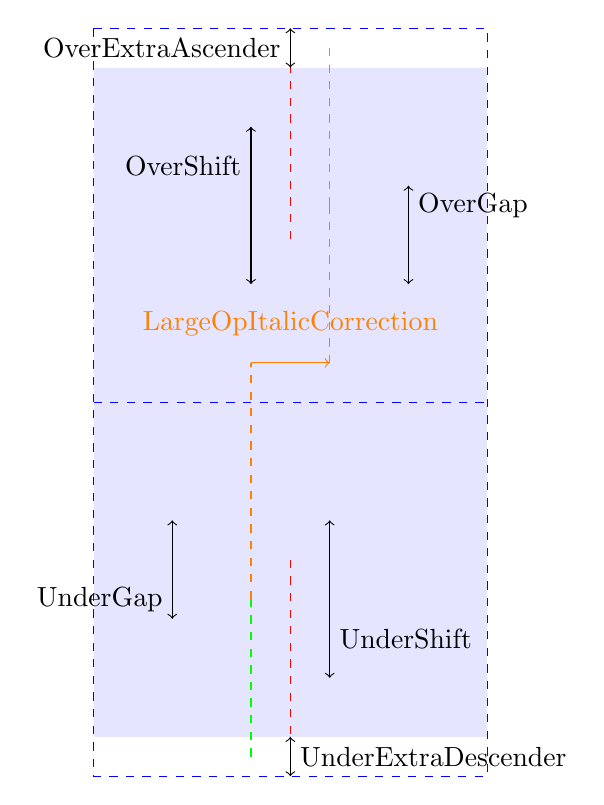
\begin{tikzpicture}[yscale=-1]

  \fill[blue!10](0,-4.25) rectangle (5,4.25);

  \MathMLBox{0.75}{3.5}{.5}{.5}{green};
  \draw[green,dashed](2,4.5)--(2,2.5);

  \MathMLBox{1.75}{-3.5}{.5}{.5}{green};
  \draw[green,dashed](3,-4.5)--(3,-2.5);

  \MathMLBox{0}{0}{1}{1}{red};
  \draw[red,dashed](2.5,-4.5)--(2.5,-2) (2.5,2)--(2.5,4.5);

  \draw[<->] (4,-1.5) -- (4,-2.5)node[right]{OverGap} -- (4,-2.75);
  \draw[<->] (2,-1.5) -- (2,-3)node[left]{OverShift} -- (2,-3.5);
  \draw[<->] (2.5,-4.25) --
             (2.5,-4.5)node[left]{OverExtraAscender} -- (2.5,-4.75);

  \draw[<->] (1,1.5) -- (1,2.5)node[left]{UnderGap} -- (1,2.75);
  \draw[<->] (3,1.5) -- (3,3)node[right]{UnderShift} -- (3,3.5);
  \draw[<->] (2.5,4.25) --
             (2.5,4.5)node[right]{UnderExtraDescender} -- (2.5,4.75);

  \draw[dashed,blue](0,-4.75) rectangle (5,4.75)
  (0,0)--(5,0);

  \draw[orange,->] (2,-.5) -- (3,-.5);
  \draw[orange] (2.5,-1)node{LargeOpItalicCorrection} ;
  \draw[orange,dashed](2,2.5) -- (2,-.5) (3,-2.5) --(3,-.5);

\end{tikzpicture}

\end{document}
